\documentclass[fleqn,leqno]{article}
\usepackage{hypertlabook}
\pdftitle{A Translator Bug}
\begin{popup}
\subsection*{A Translator Bug}

Due to a bug in the translator that we have been unable to track down,
you may have gotten an error that looks something like this:
\begin{display}
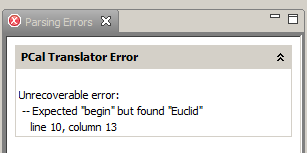
\includegraphics{translator-bug.png}
\end{display}
If that happens, just run the translator again.  (If you run the
translator by typing \textsf{control+t}, you'll have to select the
module editor first.)  That error should disappear, and the expected
error should occur.

\end{popup}
\makepopup